%!TEX TS-program = xelatex 
\documentclass[aspectratio=1610,xcolor=dvipsnames,t,compress]{beamer} 

\usepackage{listings} 
\usepackage{color} 
\usepackage{xcolor}  
\usepackage{microtype} 
\usepackage{helvet} 
\usepackage{inconsolata} 
\usepackage[framemethod=TikZ]{mdframed} 
\usepackage{graphicx} 
\usepackage{alltt}
\usepackage{sverb} 
\usepackage{verbatim} 
\usepackage{pifont} 
\usepackage{helvet} 
\usepackage{algorithm}
\usepackage{algpseudocode}

\usetheme[noflama]{sthlm}

%\usetheme{Madrid} 
%\useoutertheme{smoothbars} 
\useinnertheme{rectangles} 

\setbeamertemplate{navigation symbols}{}
\setbeamertemplate{blocks}[default] 

%\definecolor{mypurple}{rgb}{.49,0,98}
%\setbeamercolor*{palette primary}{use=structure,fg=white,bg=green}
%\usecolortheme[rgb={0.9,0.2,0.2}]{structure}
%\usecolortheme[rgb={0.6,0.1,0.1}]{structure}

%\usecolortheme[rgb={0.2, 0.2, 0.8}]{structure} 
\usecolortheme[rgb={0.0, 0.0, 0.8}]{structure} 

\usepackage{color}
\definecolor{orange}{cmyk}{0,0.4,0.8,0.2}
\definecolor{darkorange}{rgb}{.71,0.21,0.01}
\definecolor{darkgreen}{rgb}{.12,.54,.11}
\definecolor{myteal}{rgb}{.26, .44, .56}
\definecolor{gray}{gray}{0.45}
\definecolor{lightgray}{gray}{.95}
\definecolor{mediumgray}{gray}{.8}
\definecolor{inputbackground}{rgb}{.95, .95, .85}
\definecolor{outputbackground}{rgb}{.95, .95, .95}
\definecolor{traceback}{rgb}{1, .95, .95}
\definecolor{inputbg}{rgb}{0.98, 0.98, 0.98}

\usepackage{listings} 
\lstset{language=bash,
        %basicstyle=\footnotesize\ttfamily, 
        basicstyle=\small\ttfamily,
        columns=fullflexible, 
        %title=\lstname, 
        %numbers=left, stringstyle=\texttt, 
        %numberstyle={\tiny\texttt}, 
        keywordstyle=\color{blue}, 
        commentstyle=\color{darkgreen}, 
        stringstyle=\color{purple} } 


\mdfsetup{skipabove=\topskip, skipbelow=\topskip} 

\definecolor{codebg}{rgb}{0.99,0.99,0.99}

\global\mdfdefinestyle{code}{%
    frametitlerule=true,%
    frametitlefont=\small\bfseries\ttfamily,%
    frametitlebackgroundcolor=lightgray,%
    backgroundcolor=codebg,%
    linecolor=gray, linewidth=0.5pt,%
    leftmargin=0.5cm, rightmargin=0.5cm,%
    roundcorner=2pt,%
    innerleftmargin=5pt
}

\global\mdfdefinestyle{code2}{%
    topline=false,%
    bottomline=false,%
    leftline=true,%
    rightline=false,%
    backgroundcolor=codebg,%
    linecolor=gray, linewidth=0.5pt,%
    leftmargin=0.0cm, rightmargin=0.0cm,%
    innerleftmargin=1pt
}

\newcommand{\showcode}[1]{\begin{mdframed}[style=code] %
                            \lstinputlisting{#1}% 
                          \end{mdframed}% 
}

%\title[Software Engineering]{Software Architecture and Architectural Design} 
\title[Software Engineering]{Software Architectural Design} 
\subtitle{Software Engineering Process and Practice} 
\author[Michael Papasimeon]{Dr Michael Papasimeon} 
\date{28 April 2003} 

\begin{document}

\begin{frame}
    \maketitle
\end{frame} 

\begin{frame}{Engineering}
    \begin{block}{What is Engineering?} 
        \begin{quote}
            The application of scientific and mathematical principles 
            to practical ends such as the design, manufacture, and 
            operation of efficient and economical structures, machines, 
            processes, and systems. 

        \end{quote}
    \end{block} 
\end{frame}

\begin{frame}{Expectations} 
    \begin{itemize} 
        \item To learn what is meant by “Software Architecture”, 
              its importance in the software development process, 
              and how to recognise the good and bad characteristics 
              of different software architectures.
        \item Don't expect you to be world leading software designers
              at the end of this class; this will come with experience
              and lots of practice.
    \end{itemize}
\end{frame} 

\begin{frame}{What is Software Architecture?} 
    \begin{itemize}
        \item \textbf{Software architecture} refers to the theory behind the 
              actual design of computer software. 
              In the same way as a building architect sets the principles and 
              goals of a building project as the basis for the draftsman's plans, 
              so too, a software architect sets out the software architecture 
              as a basis for the actual design specifications. 
              \url{http://www.wikipedia.org/wiki/Software\_architecture}
          \item A Software Design must be \textbf{documented} to exist.
          \item A Software Architecture must describe both the 
                \textbf{STRUCTURE} and the \textbf{BEHAVIOUR} of a software system.
    \end{itemize} 
\end{frame} 

\begin{frame}{Why is Software Architecture Important?} 
    \begin{block}{Barry Boehm} 
        \emph{If a project has not achieved a system architecture, 
              including its rationale, the project should not proceed to 
              full-scale system development. 
              Specifying the architecture as a deliverable enables its 
              use throughout the development and maintenance process.
}
    \end{block}
    \begin{itemize}
        \item Mutual Communication
        \item Early Design Decisions
        \item Transferable Abstraction of a System
    \end{itemize} 
\end{frame} 

\begin{frame}{Architectural Views} 
    \begin{itemize}
        \item Functional/Logic View
        \item Code View
        \item Development/Structural View
        \item Concurrency/Process/Thread View
        \item Physical/Deployment View
        \item User Action/Feedback View
    \end{itemize} 
\end{frame} 

\begin{frame}{Why do we need a Software Architecture?} 
    \begin{itemize} 
        \item To understand how the system is intended to work.
        \item To organise software development.
        \item To foster reuse.
        \item To evolve the system.
    \end{itemize}
\end{frame} 

\begin{frame}{What influences the Software Architecture} 
    \begin{block}{Requirements and Software Patterns} 
        \begin{itemize}
            \item Requirements and use cases
            \item Experience -- previous architectures and architectural patterns
        \end{itemize}
    \end{block}
    \begin{block}{Constraints and Enablers} 
        \begin{itemize}
            \item System software
            \item Middleware (e.g. frameworks)
            \item Legacy systems
            \item Standards and policies
            \item Non functional requirements
            \item Distribution needs
        \end{itemize}
    \end{block} 
\end{frame}

\begin{frame}{Architectural Description} 
    \begin{itemize}
        \item Architecture should be developed after requirements have been 
              gathered and analysed.
        \item Architecture should be documented and should remain relatively 
              stable throughout the life of the project.
        \item Architecure may be updated, but shouldn’t grow dramatically. 
              Changes may include:
              \begin{itemize} 
                    \item Finding new abstract classes and interfaces
                    \item Adding new functionality to existing sub-systems/modules
                    \item Upgrading to new versions of re-useable components
                    \item Re-arranging the process structure.
                \end{itemize}
    \end{itemize}
\end{frame} 

\begin{frame}{Architectural Examples} 
    \begin{itemize} 
        \item Pipeline
        \item Transaction
        \item Layered
        \item Repository
        \item Client-server 
        \item Distributed computing 
        \item Peer-to-peer system 
        \item Model-View-Controller
        \item Monolithic system 
        \item Three-tier model 
        \item Structured 
        \item Component architecture
    \end{itemize}
\end{frame} 

\begin{frame}{Modular Software Design} 
    \begin{itemize} 
        \item Reduces Complexity.
        \item Facilitates Change (Easier Maintainability).
        \item Easier Implementation by encouraging parallel development.
        \item Module is the basic unit of software used in a design description.
        \item Determined using step-wise refinement (logical parts)
        \item Modules, sub-systems, components, packages, and classes are all
            software elements used for \textbf{abstraction} and \textbf{information
            hiding}~\footnote{Pressman 3rd Edition (Section 10.4 pg 332)}.
    \end{itemize} 
\end{frame} 

\begin{frame}{Levels of Abstraction} 
    \begin{itemize}
        \item Data Structures and Algorithms
        \item Classes (data structures and many algorithms)
        \item Packages/Modules (groups of related, possibly interacting classes 
              through design patterns).
        \item Modules/Subsystems (interacting modules each containing many 
              classes, but only the public interfaces interact with other modules/subsystems).
        \item Systems (systems interacting with other systems, hardware, software and human).
    \end{itemize}
    Software architecture tends to be concerned with the last two.
\end{frame} 

\begin{frame}{Module Cohesion} 
    \begin{itemize} 
        \item A measure of how functionally coherent a software module is.
        \item A software module should have \textbf{High Cohesion}.
        \item This means that a software module is concerned with 
              only doing one thing – and doing that thing well.
        \item For large modules, their components/classes should be functionally related.
    \end{itemize} 
\end{frame} 

\begin{frame}{Types of Cohesion} 
    \begin{center}
        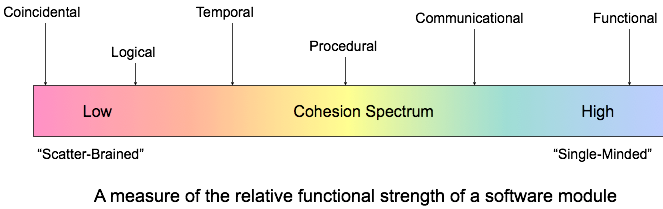
\includegraphics[width=0.65\textwidth]{cohesion} 
    \end{center} 
    \begin{block}{Software Module Cohesion...}
        \begin{itemize} 
            \item \textbf{Coincidental:} multiple, completely unrelated actions or components
            \item \textbf{Logical:} series of related actions or components (e.g. library of IO functions)
            \item \textbf{Temporal:} series of actions related in time (e.g. initialisation modules)

            \item \textbf{Procedural:} series of actions sharing sequences of steps.
            \item \textbf{Communicational:} procedural cohesion but on the same data.
            \item \textbf{Functional:} one action or function
        \end{itemize} 
    \end{block} 
\end{frame} 

\begin{frame}{Module Coupling} 
    \begin{itemize}
        \item Coupling is a measure of how inter-related or interdependent software modules are.
        \item There should be \textbf{LOW COUPLING} between software modules.
        \item This means that should be only a few well defined, 
              functionally relevant dependencies between software modules.
        \item Highly coupled software is BAD software.
(difficult to understand, maintain, debug etc…)
    \end{itemize}
\end{frame} 

\begin{frame}{Types of Coupling}
    \begin{center}
        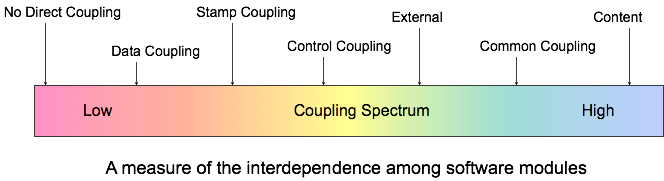
\includegraphics[width=0.6\textwidth]{coupling}
    \end{center}
    \begin{block}{Software Module Coupling...}
        \begin{itemize} 
            \item \textbf{Content:} one module directly references the content of another
            \item \textbf{Common:} both modules have access to the same global data.
            \item \textbf{Control:} One module passes the element of control to another.
        \end{itemize}
    \end{block}
\end{frame} 

\begin{frame}{Design for Reuse}
    \begin{itemize}
        \item Reusable Components/Modules are general
        \item Reusable Components are Loosely Coupled
        \item Requires High Cohesion and Published Interface
    \end{itemize}
\end{frame} 

\begin{frame}{Performance Constraints}
    \begin{itemize}
        \item Having lots of layers can result in performance issues.
        \item It is a good idea to generally design your architecture 
              with high cohesion and low coupling and then adapt it to 
              iron out performance issues.
    \end{itemize} 
\end{frame} 

\begin{frame}{Steps in creating a Software Architecture} 
    \begin{itemize}
        \item Identify major modules (or sub-systems) and sub-modules.
        \item Identify interactions with external actors and systems.
        \item Identify dependencies between modules.
        \item Determine the public classes, functions or sub-modules for each module.
        \item Identify which public classes from each module will interact with each other.
        \item Determine the interaction order between the modules.
        \item Determine how two modules will interact using experience and design patterns.
        \item Identify the methods (functions) used that will interact with other modules methods (functions).
        \item Determine the dynamic interactions (run-time)
        \item Prototype the architecture
        \item Document it.
        \item Review it.
        \item Iterate through it a couple of times to make sure it is modular, extensible, satisfies requirements (including performance etc).
        \item Compile it...
    \end{itemize}
\end{frame} 

\begin{frame}{Example Game Architecure: Module Dependencies} 
    \begin{center}
        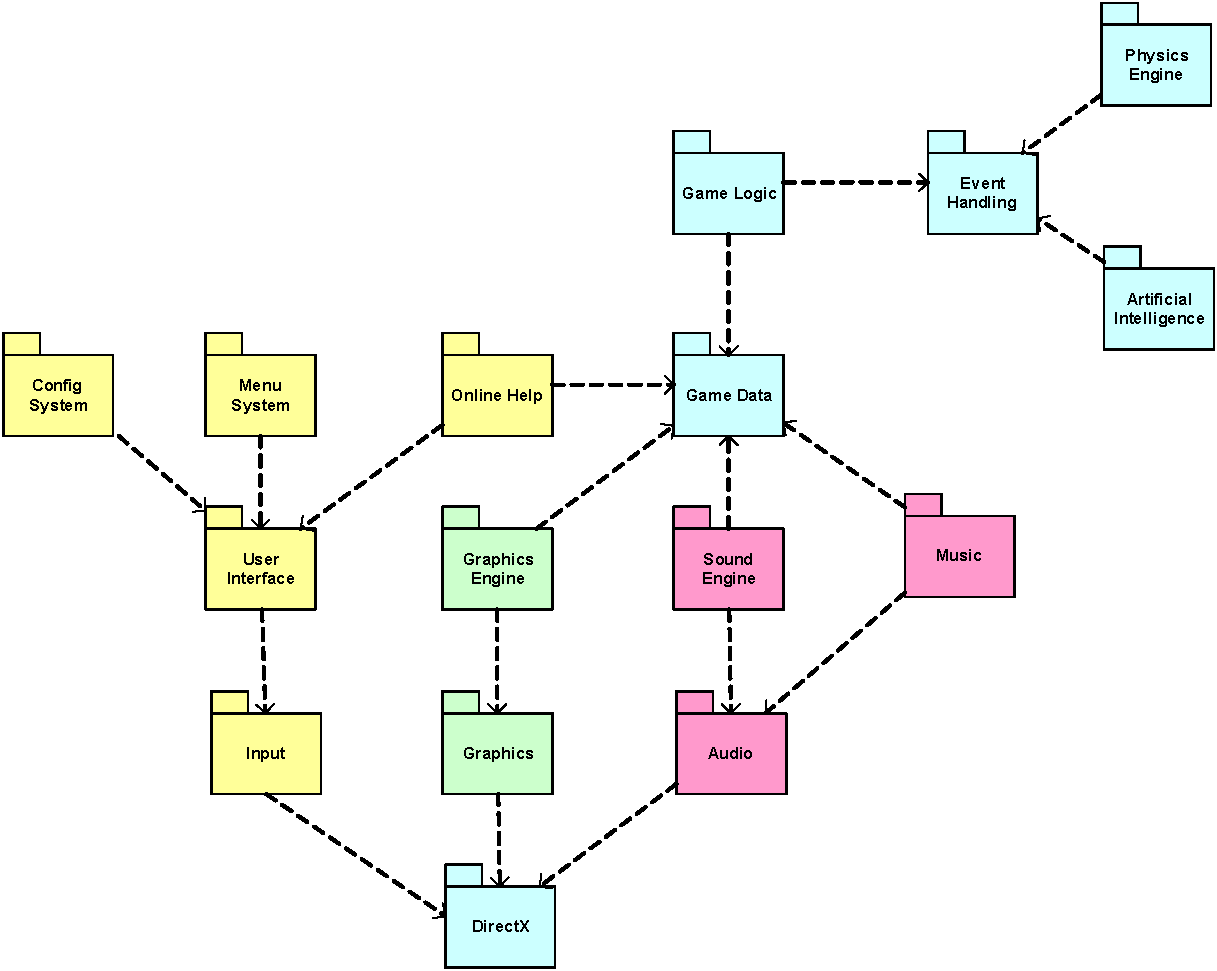
\includegraphics[width=0.65\textwidth]{game-architecture}
    \end{center}
\end{frame} 

\begin{frame}{Layered Architecture}
    \begin{center}
        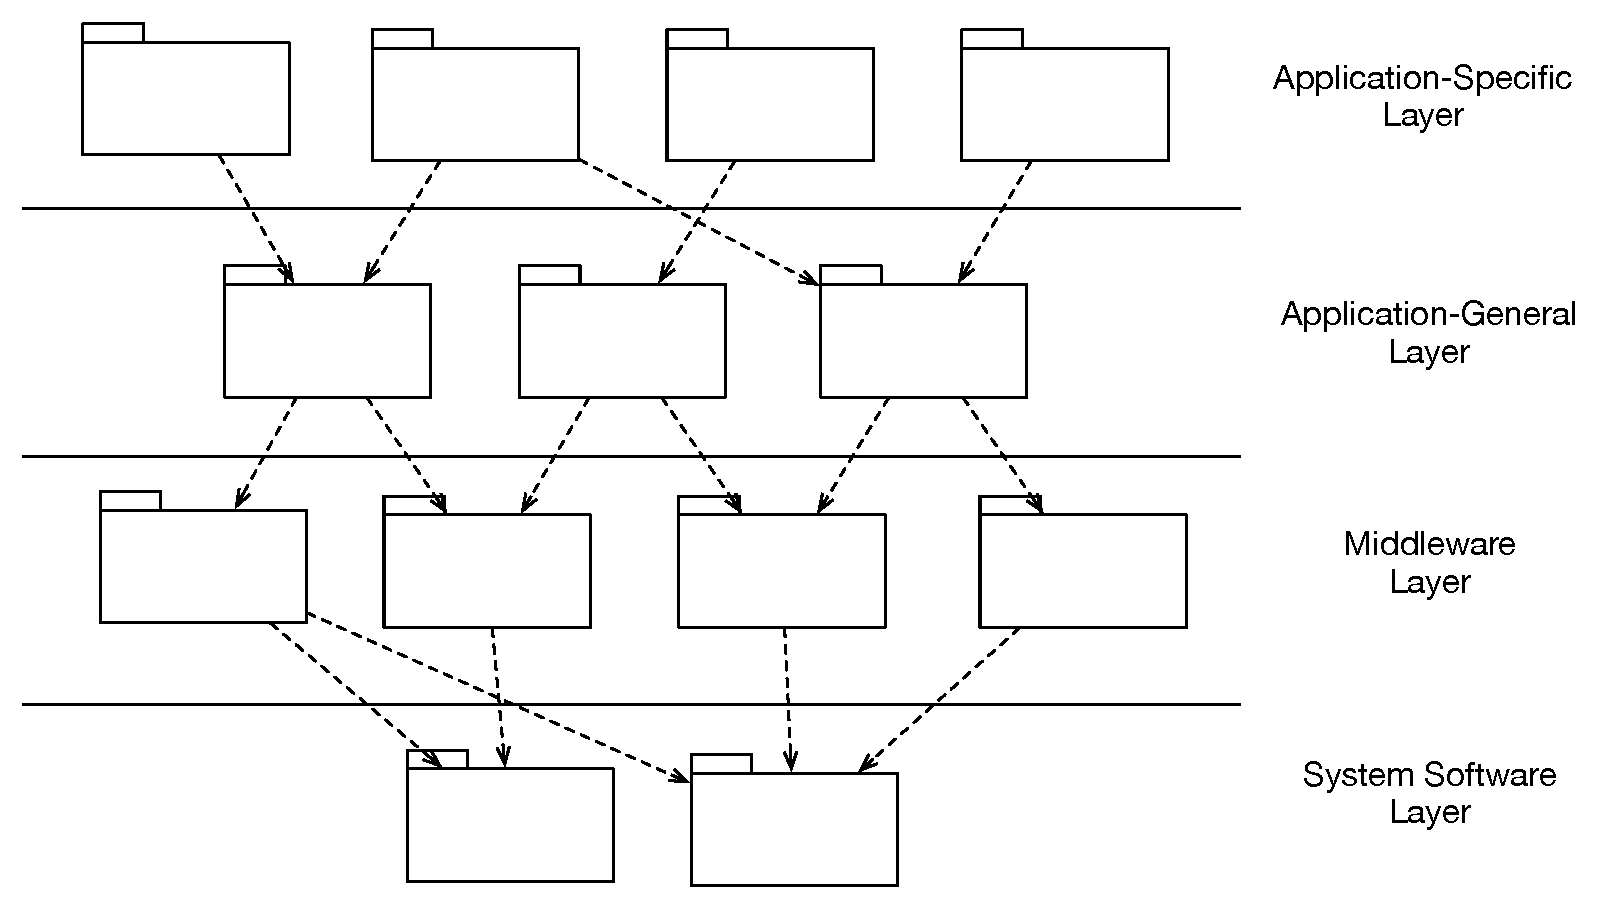
\includegraphics[width=0.9\textwidth]{layers} 
    \end{center}
\end{frame} 

\begin{frame}{Module Interfaces} 
    \begin{center}
        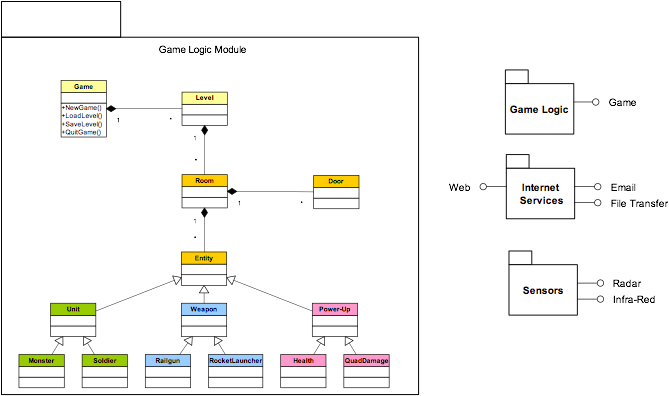
\includegraphics[width=0.7\textwidth]{module-interfaces} 
    \end{center}
\end{frame} 

\begin{frame}{Architectural Behaviour} 
    \begin{center}
        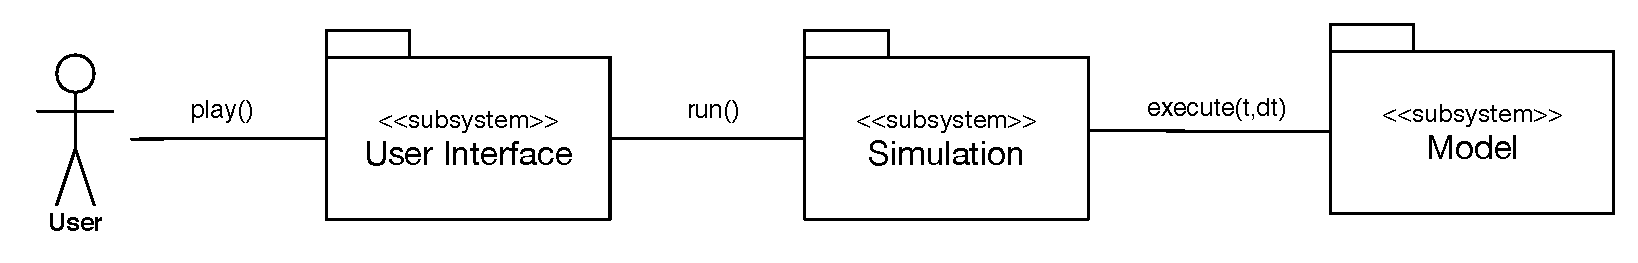
\includegraphics[width=0.9\textwidth]{behaviour} 
    \end{center} 
\end{frame} 

\begin{frame}{Detailed Design: Module Specification}
    \begin{itemize}
        \item What the function of a module is:
        \item Description of what the purpose and function of a module is.
        \item Inputs and Outputs
        \item Dependencies
        \item Errors and Exceptional Conditions
    \end{itemize} 
\end{frame} 

\begin{frame}{Some questions for the Preliminary Architectural Design Review} 
    \begin{itemize}
        \item Does the architecture satisfy the requirements?
        \item Is effective modularity achieved? 
        \item Are interfaces defined for modules and external system elements?
        \item Is the structure of the data and it’s organisation consistent 
              with the domain of the requirements?
        \item Is the structure of the data consistent with the requirements?
        \item Has maintainability been considered?
        \item Have quality factors been explicitly assessed?
    \end{itemize}
\end{frame} 

\begin{frame}{Books About Software Design}
    \begin{itemize}
        \item Design Patterns: Elements of Reusable Object Oriented Software (Gamma et. al)
        \item Pattern-Oriented Software Architecture, \\ Vol.1: 
A System of Patterns (Buschmann et. al)
        \item Software Engineering : A Practitioner’s Approach (Pressman)
        \item The Unified Software Development Process (Jacobson, Booch, Rumbaugh)
        \item Use Case Driven Object Modelling and Design with UML: A Practical Approach (Rosenberg)
        \item UML Distilled (Fowler)
        \item Analysis Patterns (Fowler)
    \end{itemize} 
    \begin{center}
        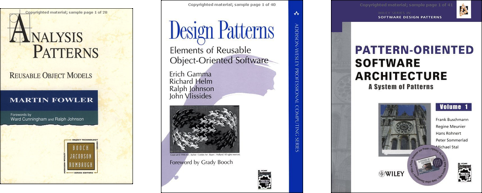
\includegraphics[width=0.6\textwidth]{books} 
    \end{center}
\end{frame} 

\begin{frame}{Books About Sofware Architecture}
    \begin{itemize}
        \item Applied Software Architecture (Hofmeister)
        \item Evaluating Software Architectures: Methods and Case Studies (Clements)
        \item Design and Use of Software Architecture (Bosch)
        \item The Software Architect’s Profession: An Introduction (Sewell et al)
        \item Software Architecture: Organizational Principles and Patterns (Dikel)
        \item Documenting Software Architectures: Views and Beyond (Clements)
        \item Software Fortresses: Modeling Enterprise Architectures (Sessions)
        \item Beyond Software Architecture: Creating and Sustaining Winning Solutions (Hohmann)
    \end{itemize}
\end{frame}

\end{document}
